\section{Results}
\begin{figure*}[!ht]            % “*”→span both columns; [!t]→force it to the top
  \centering
  % first image, take roughly half the page width:
  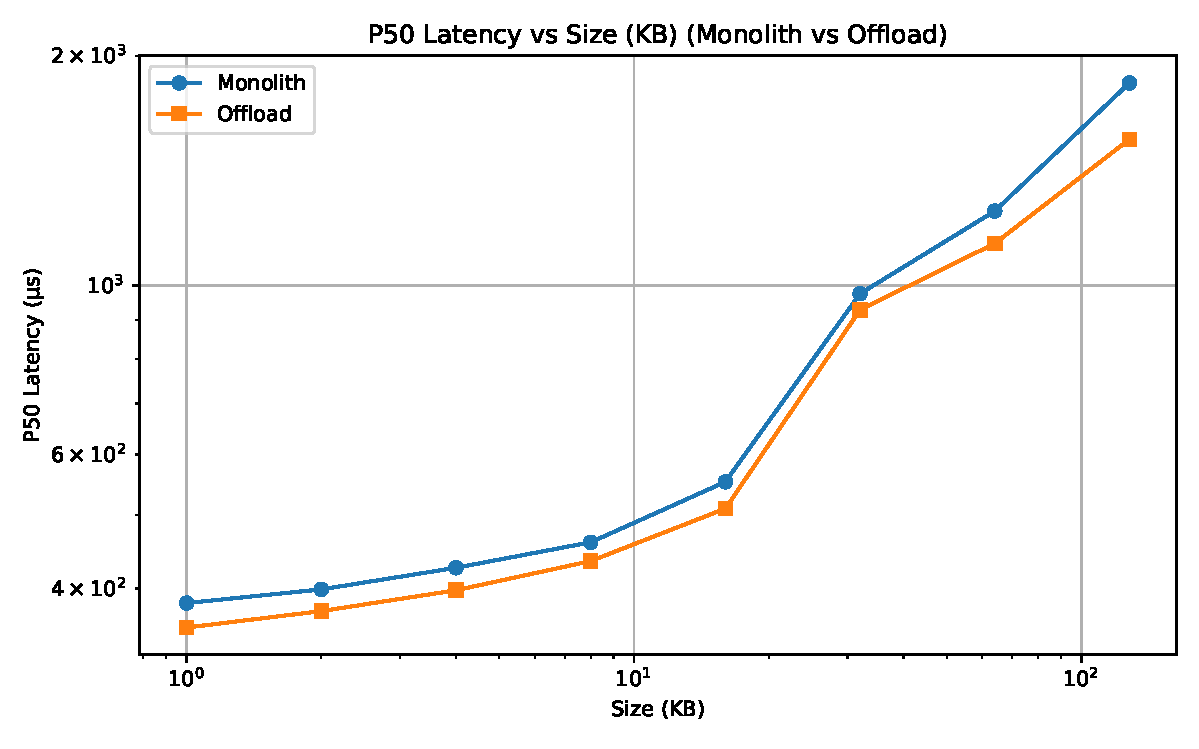
\includegraphics[width=0.48\textwidth]{size.pdf}%
  \hfill
  % second image:
  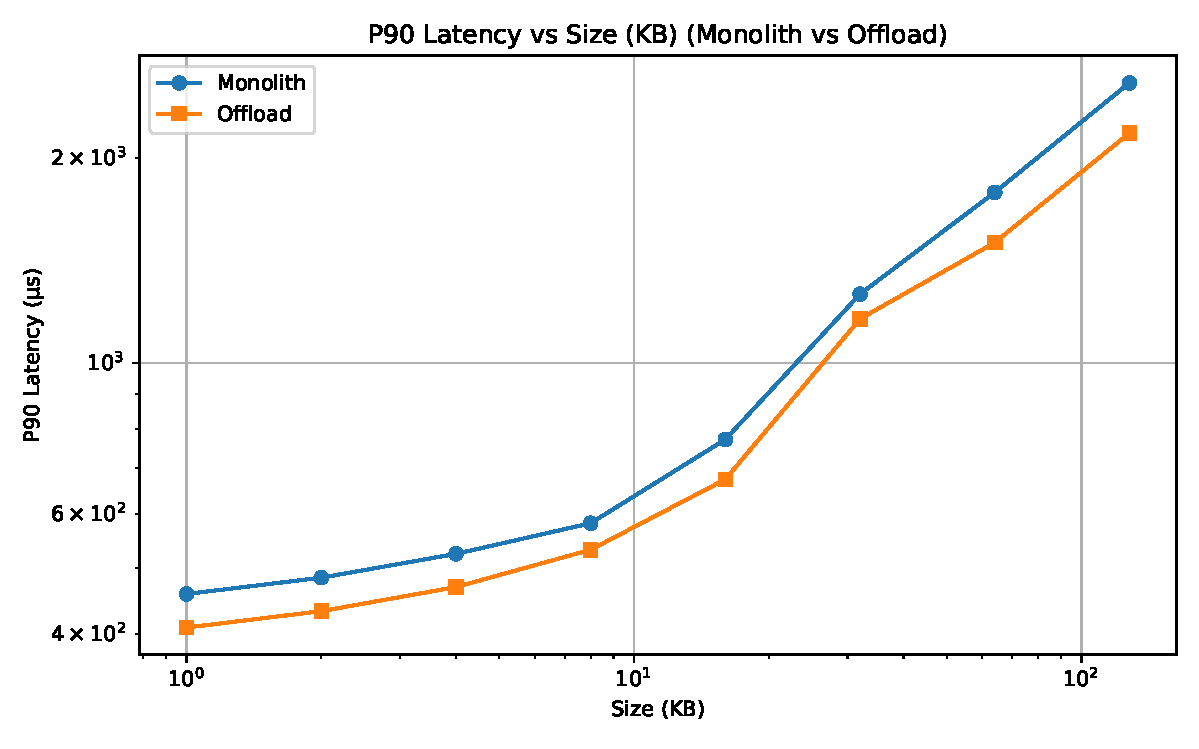
\includegraphics[width=0.48\textwidth]{size_p90.pdf}
  \caption{Median and 90th percentile latency versus the size of the input data. Sizes vary from 1KB to 128KB, with a data point at each power of two. Past 128KB, the latency increases by several orders of magnitude for both the monolithic configuration and the microservice (offload) configuration, so we omit those data points for clarity. The offered load is fixed at 4,000 requests per second. For both median and tail latency, the microservice configuration with offloaded (de)compression performs marginally better than the monolithic configuration.}
  \label{fig:size}
\end{figure*}

\begin{figure*}[!ht]            % “*”→span both columns; [!t]→force it to the top
  \centering
  % first image, take roughly half the page width:
  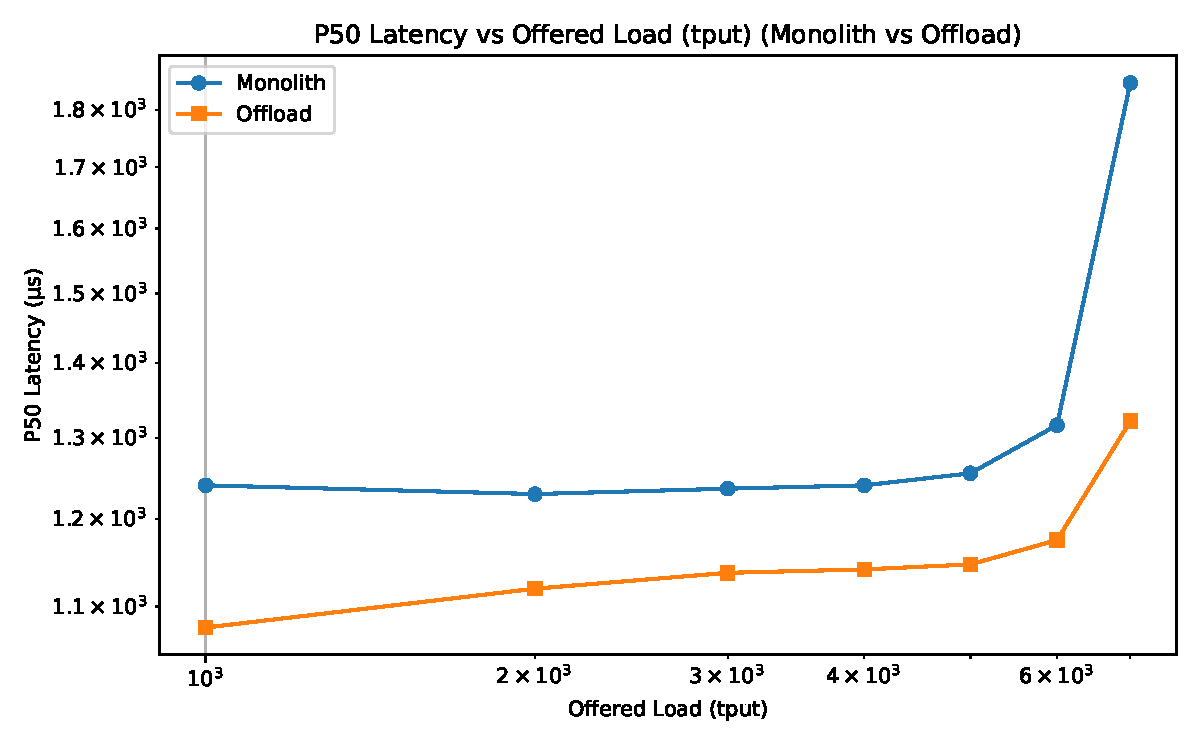
\includegraphics[width=0.48\textwidth]{p50.pdf}%
  \hfill
  % second image:
  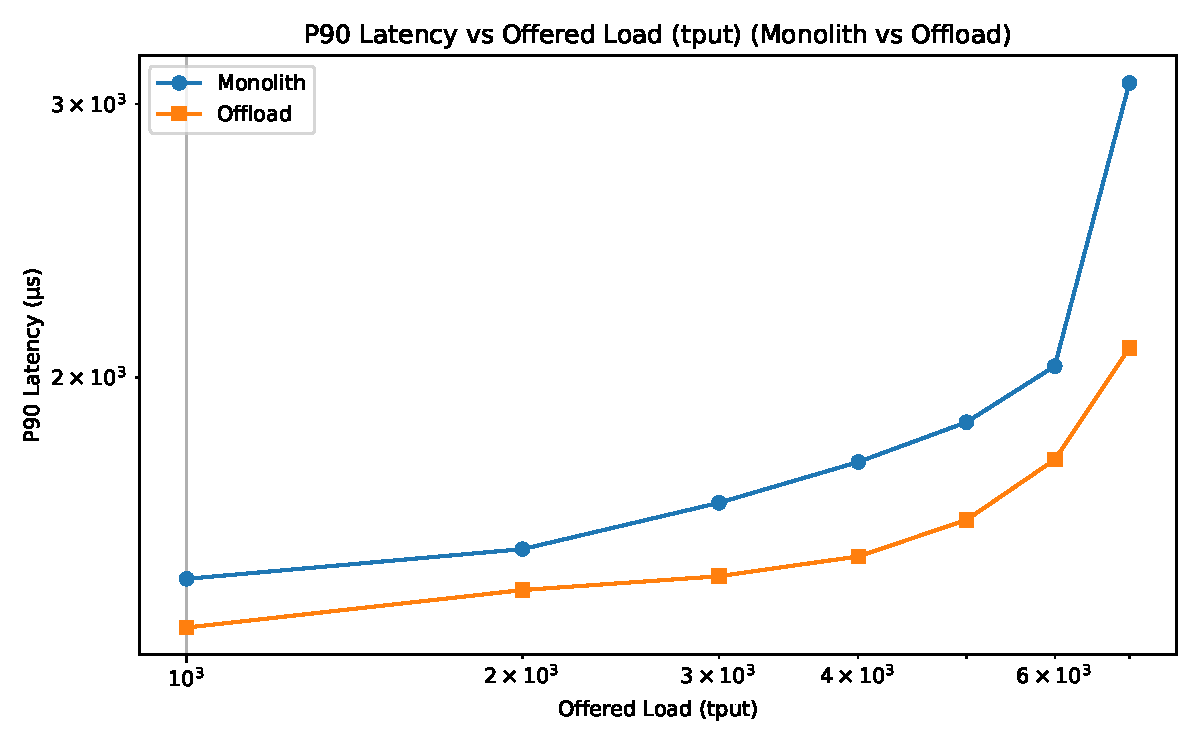
\includegraphics[width=0.48\textwidth]{p90.pdf}
  \caption{Median and 90th percentile latency versus the offered load. The load varies from 1,000 requests per second to 7,000. Past 7,000 requests per second, the latency increases by several orders of magnitude for both the monolithic configuration and the microservice (offload) configuration, so we omit those data points for clarity. The input data size is fixed at 64KB. Again, for both median and tail latency, the microservice configuration with offloaded (de)compression performs marginally better than the monolithic configuration.}
  \label{fig:tput}
\end{figure*}

\subsection{Experimental Setup}
We conduct experiments using one dual-socket server, each with a 28-core Intel Xeon Gold 5420+ CPU operating at 2.0 GHz and 256 GB of RAM. 
Hyperthreading was enabled. 
The operating system was Ubuntu 24.04. 
We pinned all containers to one socket, and we only used the IAA device local to the socket. 
The IAA was configured with 8 shared work queues and 8 engines.

\subsection{Service Configurations}
We evaluated two configurations for the compressed cache service.
\begin{enumerate}
  \item A monolithic configuration that places the frontend service and compression service in the same process and the same container. Communicating between the two services is done through a local function call. The QPL software path is used for (de)compression.
  \item A microservice configuration that splits the frontend service and compression service into separate containers, requiring that they communicate over gRPC, but offloading the (de)compression operations to the IAA.
\end{enumerate}
For both, we use Memcached as the cache implementation, which is hosted in its own container and accessed by the frontend service via gRPC. Likewise, the scheduler service is hosted in its own container and communicates with the compression service to collect operation metrics over gRPC.
